% !TEX TS-program = XeLaTex
% !TEX encoding = UTF-8 Unicode

\documentclass[UTF8]{beamer}
\usepackage{ctex, hyperref}
\usepackage[T1]{fontenc}

\usepackage[backend=biber,style=numeric-comp,sorting=none]{biblatex}
\addbibresource{ref.bib} %BibTeX数据文件及位置
\setbeamerfont{footnote}{size=\tiny} %调整注脚的文字大小

% other packages
\usepackage{latexsym,amsmath,xcolor,multicol,booktabs,calligra}
\usepackage{graphicx,pstricks,listings,stackengine}
\usepackage{pgfplots}
\pgfplotsset{width=\textwidth,compat=1.9}
\setCJKfamilyfont{myfont}{msyh.ttc}
\newcommand{\MyFont}{\CJKfamily{myfont}}
%\usepackage{auto-pst-pdf}
%\usepackage[utf8]{inputenc}

\author{\MyFont{Leyi Zhao}}
\title{\MyFont{Separating Out the Eigenvalue Densities: Computing the Jacobians}}
\subtitle{Random Matrix Theory with Its Applications}
\institute{\MyFont{School of Cyberspace}}
\date{\today}
\usepackage{hdu}

% defs
\def\cmd#1{\texttt{\color{red}\footnotesize $\backslash$#1}}
\def\env#1{\texttt{\color{blue}\footnotesize #1}}
\definecolor{deepblue}{rgb}{0,0,0.5}
\definecolor{deepred}{rgb}{0.6,0,0}
\definecolor{deepgreen}{rgb}{0,0.5,0}
\definecolor{halfgray}{gray}{0.55}

\lstset{
    basicstyle=\ttfamily\small,
    keywordstyle=\bfseries\color{deepblue},
    emphstyle=\ttfamily\color{deepred},    % Custom highlighting style
    stringstyle=\color{deepgreen},
    numbers=left,
    numberstyle=\small\color{halfgray},
    rulesepcolor=\color{red!20!green!20!blue!20},
    frame=shadowbox,
}

%%tips:
\usepackage{geometry}
\usepackage{lipsum}
\usepackage[dvipsnames,svgnames]{xcolor}
\usepackage{tcolorbox}
\tcbuselibrary{most}
\definecolor{tipscolor}{rgb}{0.77,0.72,0.65} % 莫兰迪棕色
\definecolor{OldLace}{rgb}{0.992156863, 0.9607843, 0.9019608}
% ------------------******-------------------
\newtcolorbox{tips}[2][]
{enhanced,breakable,
left=12pt,right=12pt,% 左右边距
% fonttitle=\bfseries, % 可以设置标题是否粗体
coltitle=white, % 标题字体颜色
colbacktitle=tipscolor, % 标题背景颜色
attach boxed title to top left={yshifttext=-1mm},
boxed title style={skin=enhancedfirst jigsaw,arc=1mm,bottom=0mm,boxrule=0mm},
boxrule=1pt, % 边框线宽
colback=OldLace, % 文本框背景颜色
colframe=tipscolor, % 框线颜色
sharp corners=northwest,
% drop fuzzy shadow, % 可以选择是否设置阴影效果
title=\vspace{3mm}#2,
arc=1mm,
#1}
%%


\begin{document}

%\kaishu
\MyFont
\begin{frame}
    \titlepage
    \begin{figure}[htpb]
        \begin{center}
            
\includegraphics[width=0.18\linewidth]{img/hdu-logo.jpg} %插入学校的logo,支持多种格式
        \end{center}
    \end{figure}
\end{frame}

%  

\begin{frame}
    \tableofcontents[sectionstyle=show,subsectionstyle=show/shaded/hide,subsubsectionstyle=show/shaded/hide]
\end{frame}

\section{A Two-Dimensional Example}
\begin{frame}{Spectral Theorem}
    \begin{itemize}
        \item The spectral theorem:
              \begin{align*}
                  M & = U \Lambda U^*  (unitary, symplectic) \\
                  M & = U \Lambda U^T  (orthogonal)
              \end{align*}
        \item Three ensembles:
              \begin{itemize}
                  \small
                  \item \textbf{orthogonal ensemble}: the set of $n \times n$ random $\color{red}\text{complex}$ \tetbf{symmetric} matrices
                  \item \textbf{unitary ensemble}: the set of $n \times n$ random $\color{red}\text{complex}$ \textbf{Hermitian} matrices
                  \item \textnf{symplectic ensemble}: the set of $n \times n$ random $\color{red}\text{quaternion}$ \textbf{self-dual Hermitian} matrices
              \end{itemize}
    \end{itemize}
\end{frame}


\begin{frame}{Spectral Theorem}
    \begin{itemize}
        \item 谱定理(spectral theorem)描述了厄密特矩阵(Hermitian Matrix)
        \item 谱分解常见有两种形式:
              \begin{align*}
                  M & = U \Lambda U^*  (unitary, symplectic) \\
                  M & = U \Lambda U^T  (orthogonal)
              \end{align*}
        \item 这可以被视为一种坐标系变化:$M \mapsto (\Lambda, U)$
        \item 此时可以考虑计算雅可比行列式(Jacobian):$\left|det \frac{\partial M}{\partial\left(\Lambda, U\right)}\right|$
    \end{itemize}
\end{frame}

\begin{frame}{Spectral Decomposition}
    \begin{itemize}
        \item 对于厄密特矩阵(Hermitian Matrix)的谱分解来说,其形式为:$M = U \Lambda U^*$,其中$M$为厄密特矩阵,$U$为酉矩阵(unitary matrix),$\Lambda=diag(\lambda_1, \lambda_2,\dots, \lambda_n)$
        \item 对于辛矩阵(Symplectic Matrix)的谱分解来说,
    \end{itemize}
\end{frame}

\section{监督学习}
\begin{frame}{监督学习}
    \begin{itemize}
        \item 监督学习,作为机器学习的核心范式之一,主要依赖于充分标记的数据集来训练算法。
        \item 常见的技术:支持向量机、决策树、随机森林、朴素贝叶斯、K近邻算法、神经网络、梯度提升、线性回归、逻辑回归
        \item 简述四种下游任务:
              \begin{itemize}
                  \item 文本分类
                  \item 图像识别
                  \item 机器翻译
                  \item 异常检测
              \end{itemize}
    \end{itemize}
\end{frame}

\begin{frame}{文本分类}
    \small
    \begin{itemize}
        \item 文本分类是一项自动将文本文档分类到预定义类别的任务\footfullcite{joseph2015text, horecki2015natural}
        \item 支持向量机: SVMs构建在文档类别之间的最优分隔超平面上,以分类新的未标记示例\footfullcite{khamar2013short}
        \item k-最近邻: kNN算法根据新文档与训练集中标记示例的相似性/距离来预测类别\footfullcite{tin1999automated, rennie2001improving}
    \end{itemize}
\end{frame}

\begin{frame}{图像识别}
    \begin{itemize}
        \item 经典的特征提取与分类器方法
        \item 卷积神经网络方法(CNN)

    \end{itemize}
\end{frame}

\begin{frame}{经典的特征提取与分类器方法}
    \begin{itemize}
        \item 在20世纪90年代之前传统的机器学习时代,主要使用允许特征工程和传统机器学习算法来进行图像识别。这一时期的研究者和工程师们需要大量依赖专业知识和领域经验,去手工设计识别各类目标所需的特征提取算法。这类特征通常针对不同图像识别任务定制,主要有SIFT\footfullcite{lowe1999object},HOG\footfullcite{1467360}等。
    \end{itemize}
\end{frame}

\begin{frame}{卷积神经网络方法(CNN)}
    \scriptsize
    \begin{itemize}
        \item AlexNet在深度学习模型中应用了比较深的8卷积层的神经网络,包含了卷积层,池化层,全连接层等模块,如图所示。这种网络结构的设计成为后续深度网络的范式。之后便发展出了更多使用多层感知机(MLP),卷积神经网络(CNN)等的模型来进行端到端的图像特征学习和分类\footfullcite{10.1145/3065386}。

              \begin{figure}[H]
                  \centering
                  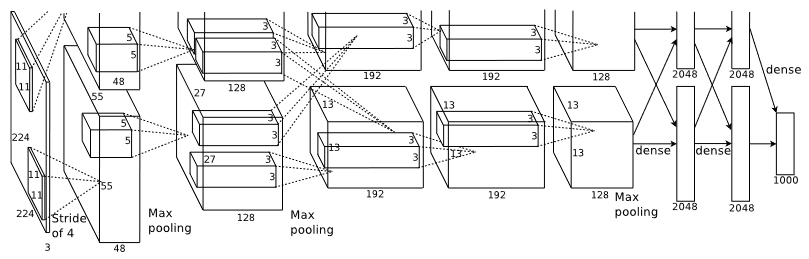
\includegraphics[width=0.8\textwidth]{img/2-Image Recognition/4.jpg}
              \end{figure}

        \item AlexNet的成功启示了后续深度学习模型对于层次化特征学习的重要性,并为图像识别任务提供了一种强大的架构范例。
              % \footfullcite{simonyan2014very}。
    \end{itemize}
\end{frame}

\begin{frame}{卷积神经网络方法(CNN)}
    \scriptsize
    \begin{itemize}
        \item GoogLeNet在图像识别中采用了独特的Inception模块以及一系列创新性的设计,其处理过程充分利用了多尺度特征的丰富性。总体而言,GoogLeNet是一种注重了模型的深度、宽度和计算效率的模型\footfullcite{szegedy2015going}。

              \begin{figure}[H]
                  \centering
                  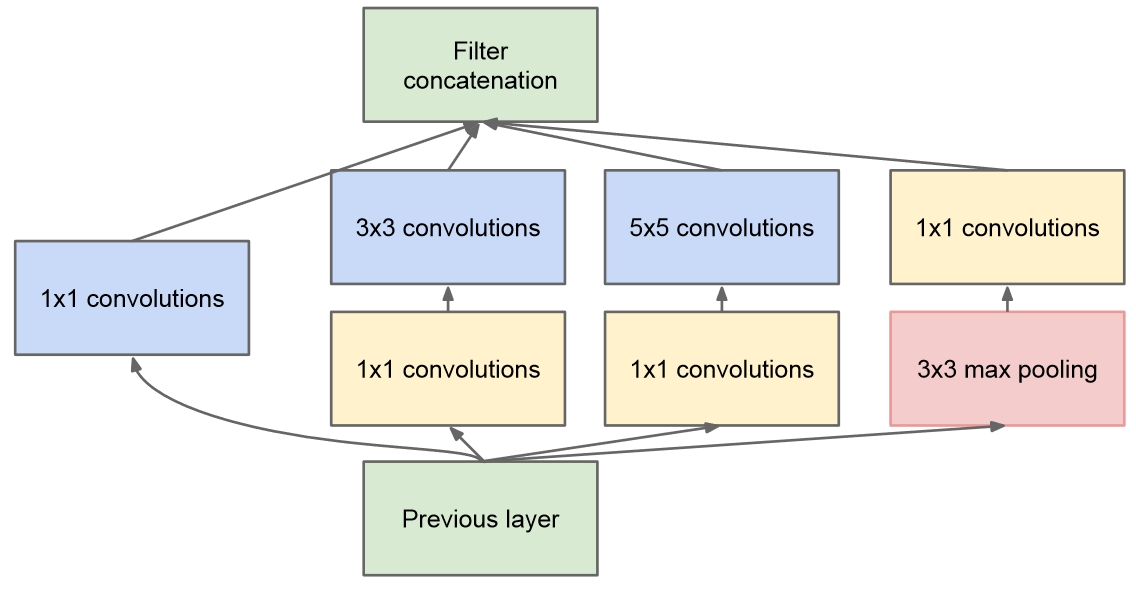
\includegraphics[width=0.8\textwidth]{img/2-Image Recognition/5.jpg}
              \end{figure}
    \end{itemize}
\end{frame}

\begin{frame}{机器翻译}
    \begin{itemize}
        \item 基于规则的机器翻译(RBMT)
        \item 统计机器翻译(SMT)
        \item 神经机器翻译(NMT)
        \item 深度强化学习机器翻译(DRLMT)
    \end{itemize}
\end{frame}

\begin{frame}{基于规则的机器翻译(RBMT)}
    \begin{itemize}
        \item RBMT是早期机器翻译方法之一,它的发展可以追溯到20世纪60年代和70年代。如Fakhrahmad等人\footfullcite{fakhrahmad2012new}于2012年针对词义消歧(WSD)这一机器翻译过程中最具挑战性的任务,提出各种监督和无监督学习方法来解决这一问题。近年最新的研究包括Chauhan等人\footfullcite{chauhan2023rule}提出的基于规则的模糊计算方法在印地语机器翻译中的自监督情感极性分类和词义消歧方面的应用
    \end{itemize}
\end{frame}

\begin{frame}{统计机器翻译(SMT)}
    \begin{itemize}
        \item 基于监督学习的统计机器翻译(SMT)是一种传统的机器翻译方法,它使用大量的双语平行语料来训练模型,包括源语言和目标语言之间的句子对。
        \item González-Rubio等人\footfullcite{gonzalez2014cost}提出了一个用于计算机辅助翻译的成本敏感主动学习框架,其目标是使翻译过程尽可能轻松。与传统的主动学习场景不同,该论文所提出的主动学习框架的设计不仅是为了最小化用户必须监督的翻译数量,还包括最小化每个翻译的监督难度。
    \end{itemize}
\end{frame}

\begin{frame}{神经机器翻译(NMT)}
    \scriptsize
    \begin{itemize}
        \item 开发低资源语言翻译技术至关重要,已经成为神经机器翻译中的一个热门研究领域。shi等人\footfullcite{shi2022low}在2022发表的一篇综述类论文中对低资源NMT中现有的深度学习技术进行了全面的回顾,展示了研究现状及一些广泛使用的低资源数据集,并将这些方法分解为七个类别以总结不同方法之间的共同特点
        \item 神经机器翻译在过去几年中取得了显著的进展,已成为机器翻译领域的主流方法,但近年更具突破性模型是监督学习下的SMT与NMT结合,Razaq等人的研究\footfullcite{razaq2023improving}展示了这一成果,其研究背景为在短语生成(PG)中,自然语言中的句子被转换成一个具有不同句法结构但具有相同语义的新句子。
    \end{itemize}
\end{frame}

\begin{frame}{异常检测}
    \begin{itemize}
        \item 传统监督学习方法
        \item 深度学习方法
        \item 应用领域
    \end{itemize}
\end{frame}

\begin{frame}{传统监督学习方法}
    \begin{itemize}
        \item 早在2009年,Babenko等人提出了一种基于“多实例学习(Multiple Instance Learning, MIL)”的方法,该方法具有潜力应用于异常检测任务\footfullcite{5206737}
        \item Babenko等人的研究提出了一种具有实时性能的多实例学习算法,用于目标跟踪\footfullcite{5206737}。
    \end{itemize}
\end{frame}

\begin{frame}{深度学习方法}
    \begin{itemize}
        \item 一项名为"Deep Learning Anomaly Detection Method in Textual Data"的研究,由Amir Jafari于2022年提出,探讨了如何结合深度学习和传统机器学习算法来检测和识别文本中的异常\footfullcite{jafari2022deep}。该研究利用深度学习模型和Transformer架构,将文本数据转化为数值表示,提供了关于文本数据的关键上下文信息。
    \end{itemize}
\end{frame}

\begin{frame}{应用领域}
    \scriptsize
    \begin{itemize}
        \item 在2017年举行的KDD Workshop on Anomaly Detection in Finance中,研究人员和从业者聚集在一起,讨论了这些新方法和解决方案\footfullcite{DBLP:conf/kdd/AnandakrishnanK17}。
        \item 一篇题为"Deep Learning based pipeline for anomaly detection and quality enhancement in industrial binder jetting processes"的研究,由Alexander Zeiser等人于2022年提出,探讨了在工业制造中使用深度学习进行异常检测和质量提升的方法\footfullcite{zeiser2022deep}。
        \item 一篇题为"Cybersecurity Vital Signs: The Role of Anomaly Detection on Insider Threat Triage"的研究,由Karla Clarke和Yair Levy于2019年提出,探讨了异常检测在内部威胁检测中的重要作用\footfullcite{Clarke2019CybersecurityVS}。
        \item 一项名为"Medical Healthcare System Based on Wireless Body Area Networks: The Importance of Anomaly Detection"的研究,由Hayder Hassaballah、Rashid Fayadh和Bushra AlHayali于2020年提出,旨在探讨在医疗WBSN系统中使用异常检测的现代框架\footfullcite{Medical_Healthcare}。
    \end{itemize}
\end{frame}

\begin{frame}
    \begin{center}
        {\Huge\calligra Thanks!}
    \end{center}
\end{frame}

\end{document}